\documentclass[a4paper,12pt]{article}
\usepackage[utf8]{inputenc}
\usepackage[spanish]{babel}

\usepackage{graphicx}
\usepackage{geometry}
\usepackage{multicol}
\usepackage{tikz}
\usepackage{lmodern}
\usepackage{caption}
\usepackage{float}
\usepackage{enumitem}
\usepackage{multirow}
\usepackage{circuitikz}
\usepackage{amsmath}
\usepackage{siunitx}
\usepackage{textcomp}
\geometry{left=2cm,right=2cm,top=2cm,bottom=2cm}
\pagestyle{empty}

\begin{document}

\begin{minipage}[t]{0.74\textwidth}
    \fbox{%
        \begin{minipage}[t][25cm][t]{\textwidth}
            \vspace*{1.5cm}
            \begin{center}
                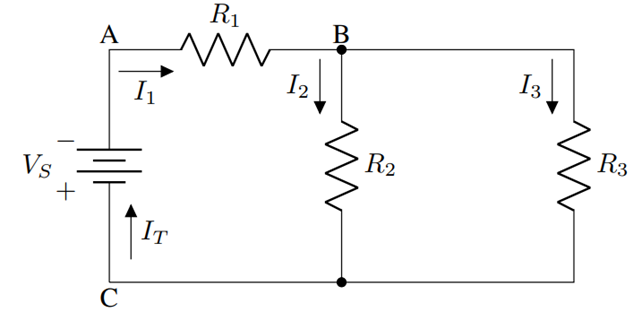
\includegraphics[width=1\textwidth]{imagenes/circuito.png} \\[1.5cm]
                \Huge \textbf{Trabajo práctico Nº1}
            \end{center}
            \vfill
            \normalsize
            \begin{itemize}[left=1em]
            \item \textbf{Autores:}
            \begin{itemize}[left=1em]
                \item Marcos Acevedo - Leg. 402898 (Coordinador)
                \item Mariano Condori - Leg. 406455 (Operador)
                \item Ignacio Perea - Leg.406265 (Documentador)
                \item Gonzalo Filsinger - Leg. 403797(Documentador)
            \end{itemize}
            \vspace{0.5cm}
            \item \textbf{Año Lectivo:} 2025
            \item \textbf{Curso:} 3R1 
            \item \textbf{Asignatura:} Dispositivos Electrónicos. 
            \item \textbf{Institución:} Universidad Tecnológica Nacional - Facultad Regional de Córdoba.
            \end{itemize}
        \end{minipage}
    }
\end{minipage}
\hfill
\begin{minipage}[t]{0.23\textwidth}
    \fbox{%
        \begin{minipage}[t][25cm][t]{\textwidth}
            \begin{center}
                \vspace{0.5cm}
                
\includegraphics[width=2.5cm]{imagenes/utnlogo.png} \\[1cm]
                \vspace{1cm}
                {\Huge
                \begin{tabular}{c}
                    \textbf{U} \\
                    \textbf{T} \\
                    \textbf{N} \\\\
                    \textbf{F} \\
                    \textbf{R} \\
                    \textbf{C}
                \end{tabular}
                }
            \end{center}
        \end{minipage}
    }
\end{minipage}

\section{Actividades}
\subsection{Calculos}
\paragraph{Para el siguiente circuito se nos pide obtener los valores de $i_1$, $i_2$, $i_3$ junto a $v_{R1}$, $v_{R2}$ y $v_{R3}$,  sabiendo que:}
\begin{itemize}
    \item $V_s = 10V$
    \item $R_1= \SI{10}{\kilo\ohm}$
    \item $R_2= \SI{4.7}{\kilo\ohm}$
    \item $R_3= \SI{3.3}{\kilo\ohm}$
\end{itemize}
\paragraph{}
\paragraph{}
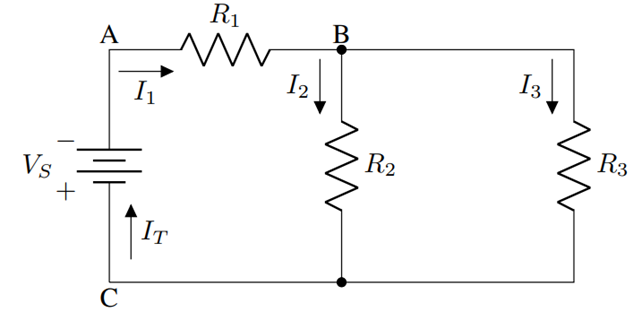
\includegraphics[width=10cm]{imagenes/circuito.png}\\[1.5cm]

\paragraph{Calculo de corriente total:}
\paragraph{}
Para resolver el ejercicio utilizaremos las leyes de Kirchhoff y ley de Ohm, primero debemos obtener la resistencia total del circuido para calcular la corriente total mediante ley de Ohm.

\begin{equation*}
    i_T = \frac{V_T}{R_T}
\end{equation*}

\vspace{1cm}

Se puede observar que las resistencias $R_2$ y $R_3$ están en paralelo por lo que calculamos a ambas de la siquiente forma:

\begin{equation*}
    R_{23} = R_2 || R_3 = \frac{1}{\frac{1}{R_2}+\frac{1}{R_3}}
\end{equation*}

Reemplazando obtenemos:

\begin{align*}
      R_{23} = \frac{1}{\frac{1}{\SI{4.7}{\kilo\ohm}}+\frac{1}{\SI{3.3}{\kilo\ohm}}} \\[0.5cm]
      R_{23} = \frac{1}{\frac{800}{1551}} \\[0.5cm]
      R_{23} = \frac{1551}{800}\times10^3 \approx \SI{1.94}{\kilo\ohm}
\end{align*}

Ahora vemos que $R_{23}$ esta en serie con $R_1$, por lo cual:

\begin{align*}
    R_T = R_1 + R_{23} \\[0.5cm]
    R_T = \SI{10000}{\ohm} + \frac{1551}{800}  \\[0.5cm]
    R_T = \frac{9551}{800} \times10^3 \approx \SI{11.94}{\kilo\ohm}
\end{align*}

Ahora que tenemos $R_T$, y teníamos como dato el voltaje total, siendo este el de la fuente, estamos en condiciones de calcular la corriente total:

\begin{align*}
    i_T = \frac{10V}{\frac{9551}{800} \times 10^3}\\[0.5cm]
    i_T = \frac{8}{9551} \approx 837,6 \mu A 
\end{align*}

\paragraph{Calculos de $i_1$, $i_2$ e $i_3$:}
\paragraph{}
\vspace{0.5cm}

Primero debemos empezar calculando la caida de tencion de cada resistencia, para asi calcular la corriente, para ello utilizaremos ley de Ohm:

\begin{align*}
    v_{R1} = R_1 \cdot i_T \\[0.5cm]
    v_{R1} = \SI{10}{\kilo\ohm} \cdot\frac{8}{9551}A\\[0.5cm]
    v_{R1} = \frac{80000}{9551} \approx 8,37 V
\end{align*}

Para $R_2$ y $R_3$ podemos obsevar que se encuentran en paralelo, por lo que la caida de tencion que hay en ambas son iguales, de esta forma solo calculamos una de ellas.

\begin{align*}
    v_{R2} &= V_T - v_{R1}\\[0.5cm]
    v_{R2} &= 10V - \frac{80000}{9551}\\[0.5cm]
    v_{R2} &= v_{R3} = \frac{15510}{9551} \approx 1,63V 
\end{align*}

\vspace{0.5cm}

Ahora podemos calcular los valores de corrientes respectivos a cada resistencias usando la Ley de Kirchhoff para corriente:\\

Sabemos que en el nodo  B la suma de las corrientes es 0, por lo que\\

$$i_T - i_1 - i_2 = 0$$ \\

y por ley de Ohm sabemos que:

$$i_2 = \frac{v_{R2}}{R2}$$\\

Calculando obtenemos

$$i_2 = \frac{33}{95510} \approx 345,5\mu A$$\\

Ahora calculamos la corriente restante.

\begin{align*}
    i_3 &= i_T - i_2 \\[0.5cm]
    i_3 &= \frac{8}{9551} - \frac{33}{95510}\\[0.5cm]
    i_3 &= \frac{47}{95510} \approx 492,1 \mu A
\end{align*}

\paragraph{}

Resumiendo en un cuadro:\\

\vspace{0.5cm}


\begin{table}[h]  % Intenta colocar la tabla "aquí" (here)
\centering
\begin{tabular}{|l|c|c|c|c|}
\hline
                &  $V_s$&  $R_1$&  $R_2$& $R_3$\\ \hline  
         Tensión&  10V&  8,37V&  1,63V& 1,63V\\ \hline  
         Corriente&  $837,6 \mu A$&  $837,6 \mu A$&  $345,5 \mu A$& $492,1 \mu A$\\ \hline 
\end{tabular}
\end{table}

\vspace{0.5cm}

\subsection{Simulación}

Para la simulación utilizaremos LTSpice, que es un software de simulación de circuitos electrónicos.
\\
Version Usada: 24.1.5

\vspace{0.5cm}
Primero armamos el circuito, quedandonos de la siguiente forma:\\[0.5cm]

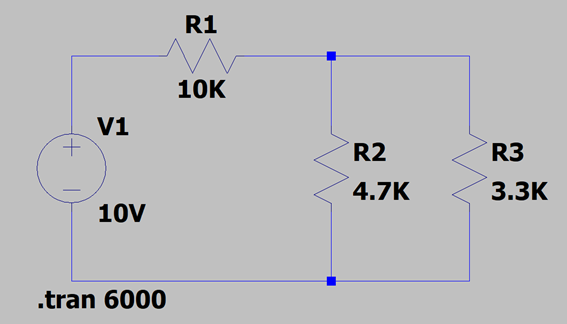
\includegraphics[width=10cm]{imagenes/cirbuitoltspice.png}\\[1.5cm]

Al simularlo obtenemos:\\

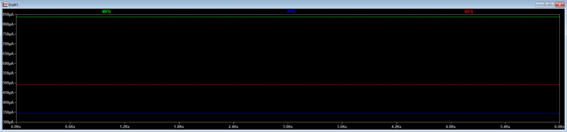
\includegraphics[width=15cm]{imagenes/simulacionresultado.png}\\[1.5cm]

Obteniendo como valores de corriente los siguientes numeros:\\

Cabe recalcar que los datos a leer sería el numero que figura en el recuadro Vert., ya que dicha medida representa el amperaje de la resistencia especificada.

\begin{figure}[H]
    \centering
    \begin{minipage}{0.31\textwidth}
        \centering
        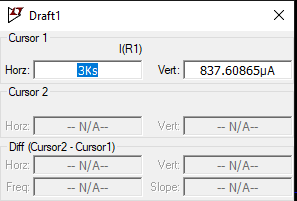
\includegraphics[width=\linewidth]{imagenes/i1resultado.png}
        \caption*{Corriente $i_1$}
    \end{minipage}
    \hfill
    \begin{minipage}{0.31\textwidth}
        \centering
        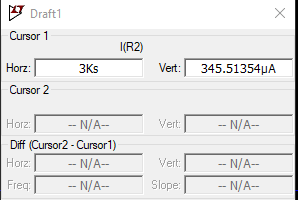
\includegraphics[width=\linewidth]{imagenes/i2resultado.png}
        \caption*{Corriente $i_2$}
    \end{minipage}
    \hfill
    \begin{minipage}{0.31\textwidth}
        \centering
        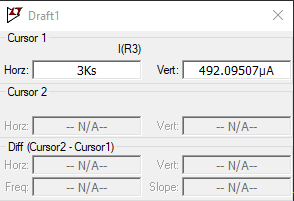
\includegraphics[width=\linewidth]{imagenes/i3resultado.png}
        \caption*{Corriente $i_3$}
    \end{minipage}
\end{figure}

\vspace{2cm}

\begin{figure}[H]
    \centering
    \begin{minipage}{0.4\textwidth}
        \centering
        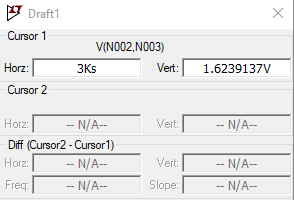
\includegraphics[width=\linewidth]{imagenes/corrientei1lt.png}
        \caption*{Tensión $i_1$}
    \end{minipage}
    \hfill
    \begin{minipage}{0.4\textwidth}
        \centering
        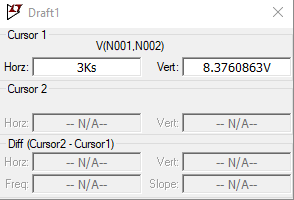
\includegraphics[width=\linewidth]{imagenes/corrientei2lt.png}
        \caption*{Tensión $i_2$}
    \end{minipage}
\end{figure}

\vspace{0.1cm}

\subsection{Medición}

\paragraph{Informacion de Instrumentos Usados:} 

\begin{itemize}
    \item Multimetro Marca: Uni-T
    \item Modelo: UT70A
    \item Error de medición:


\paragraph{}

\vspace{0.1cm}

\renewcommand{\arraystretch}{1.5}

\begin{table}[h]
    \centering
    \begin{tabular}{|>{\centering\arraybackslash}p{0.3\linewidth}|>{\centering\arraybackslash}p{0.3\linewidth}|>{\centering\arraybackslash}p{0.3\linewidth}|} \hline 
         Tensión&  Corriente& Resistencia\\ \hline 
         $\stackrel{+}{-} 0.5$ \%  &  $\stackrel{+}{-} 0.8$ \% & $\stackrel{+}{-} 0.8$ \% \\ \hline 
         +1&  +1& +1\\ \hline
    \end{tabular}
 
\end{table}

\item Valores reales de las resistencias:

\begin{figure}[H]
    \centering
    \begin{minipage}{0.35\textwidth}
        \centering
        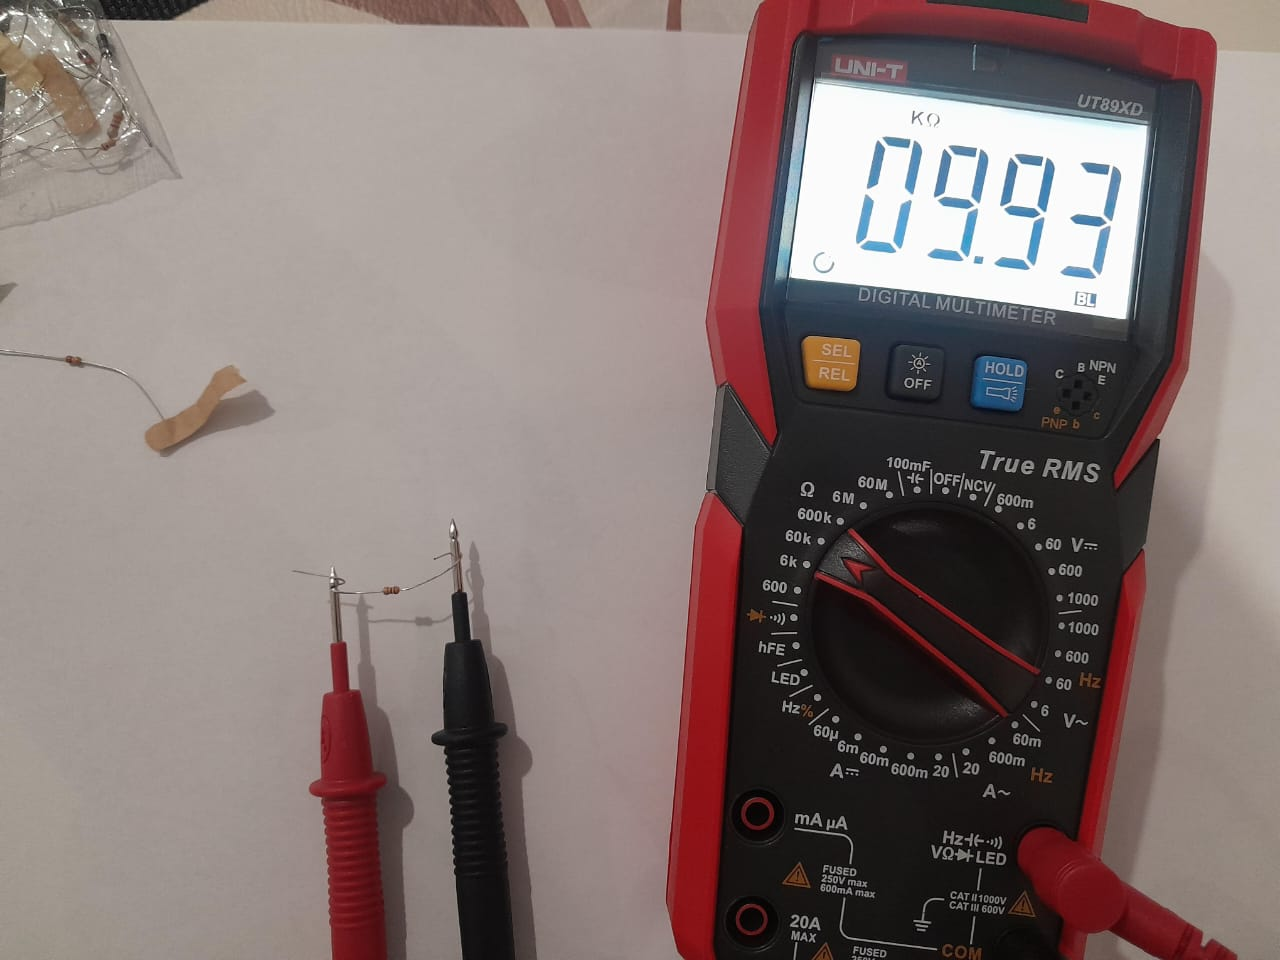
\includegraphics[width=\linewidth]{imagenes/r1.jpg}
        \caption*{$R_1$}
    \end{minipage}
    \hfill
    \begin{minipage}{0.35\textwidth}
        \centering
        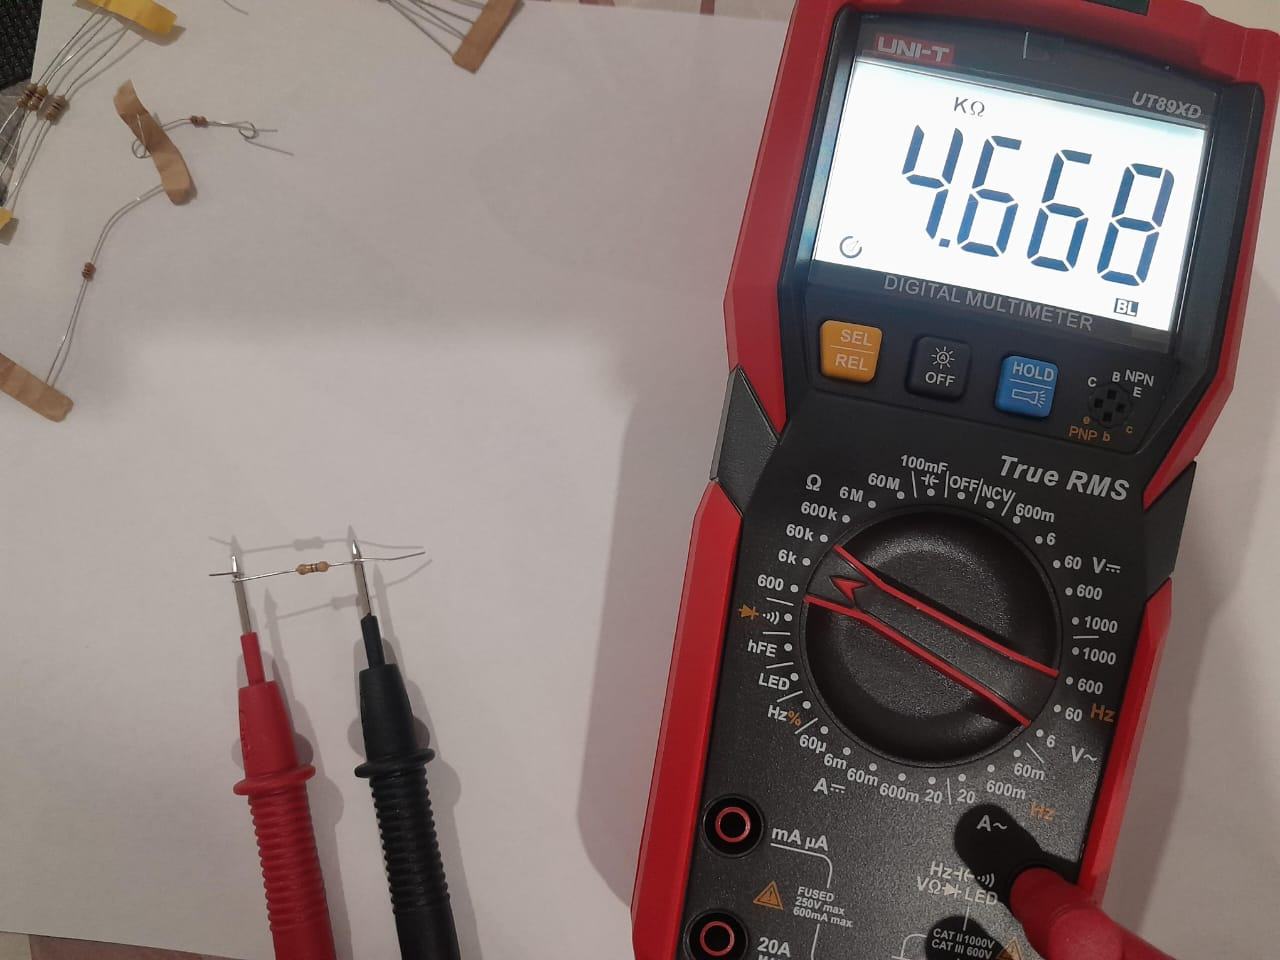
\includegraphics[width=\linewidth]{imagenes/r2.jpg}
        \caption*{$R_2$}
    \end{minipage}
    \hfill
    \begin{minipage}{0.35\textwidth}
        \centering
        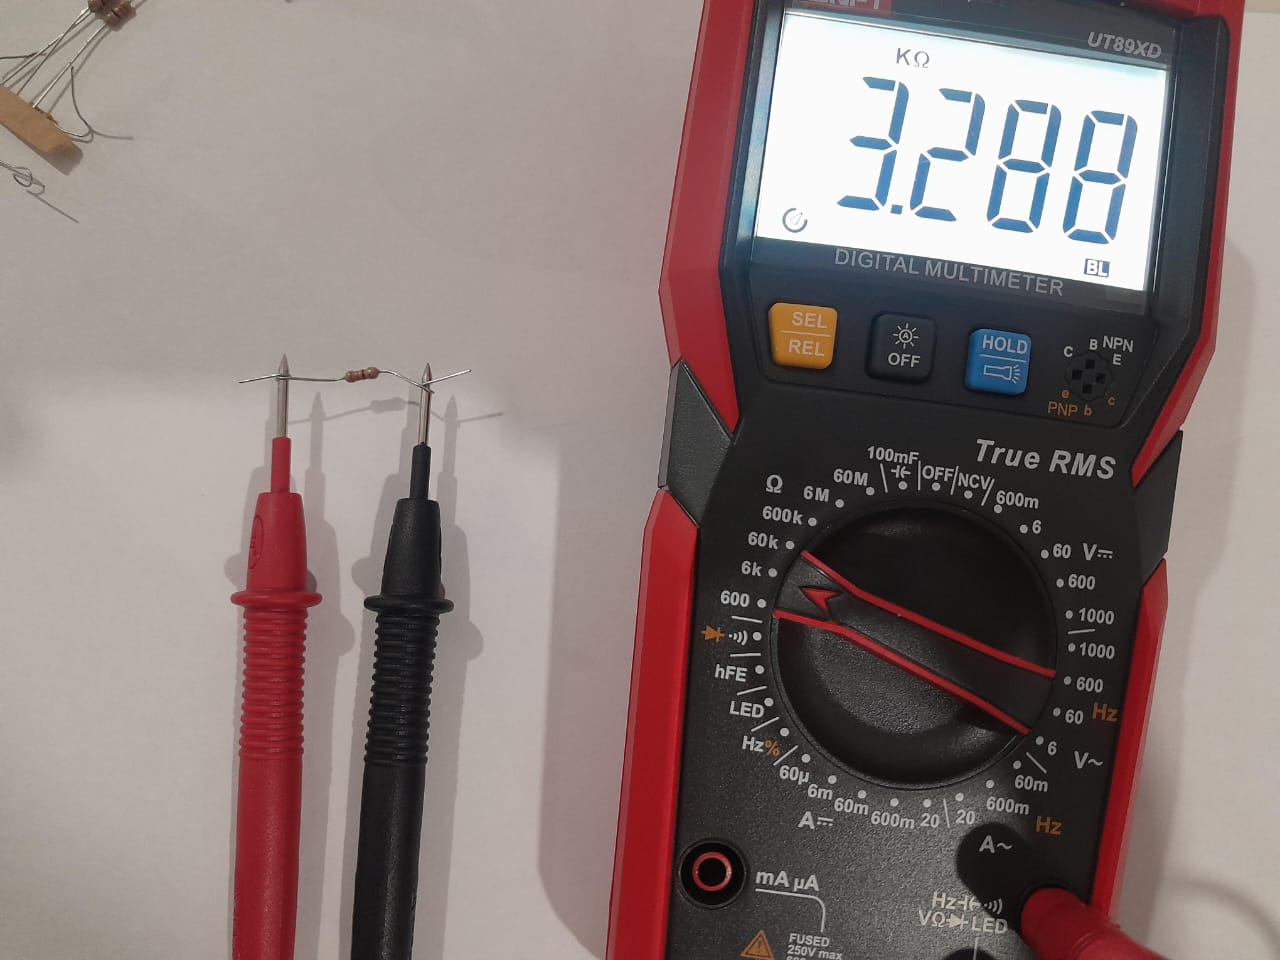
\includegraphics[width=\linewidth]{imagenes/r3.jpg}
        \caption*{$R_3$}
    \end{minipage}
\end{figure}

\end{itemize}

\begin{figure}[H]
    \centering
    \begin{minipage}{0.40\textwidth}
        \centering
        \includegraphics[width=\linewidth]{imagenes/tensionfuente.jpg}
        \caption*{Tensión de la fuente}
    \end{minipage}
    \hfill
    \begin{minipage}{0.40\textwidth}
        \centering
        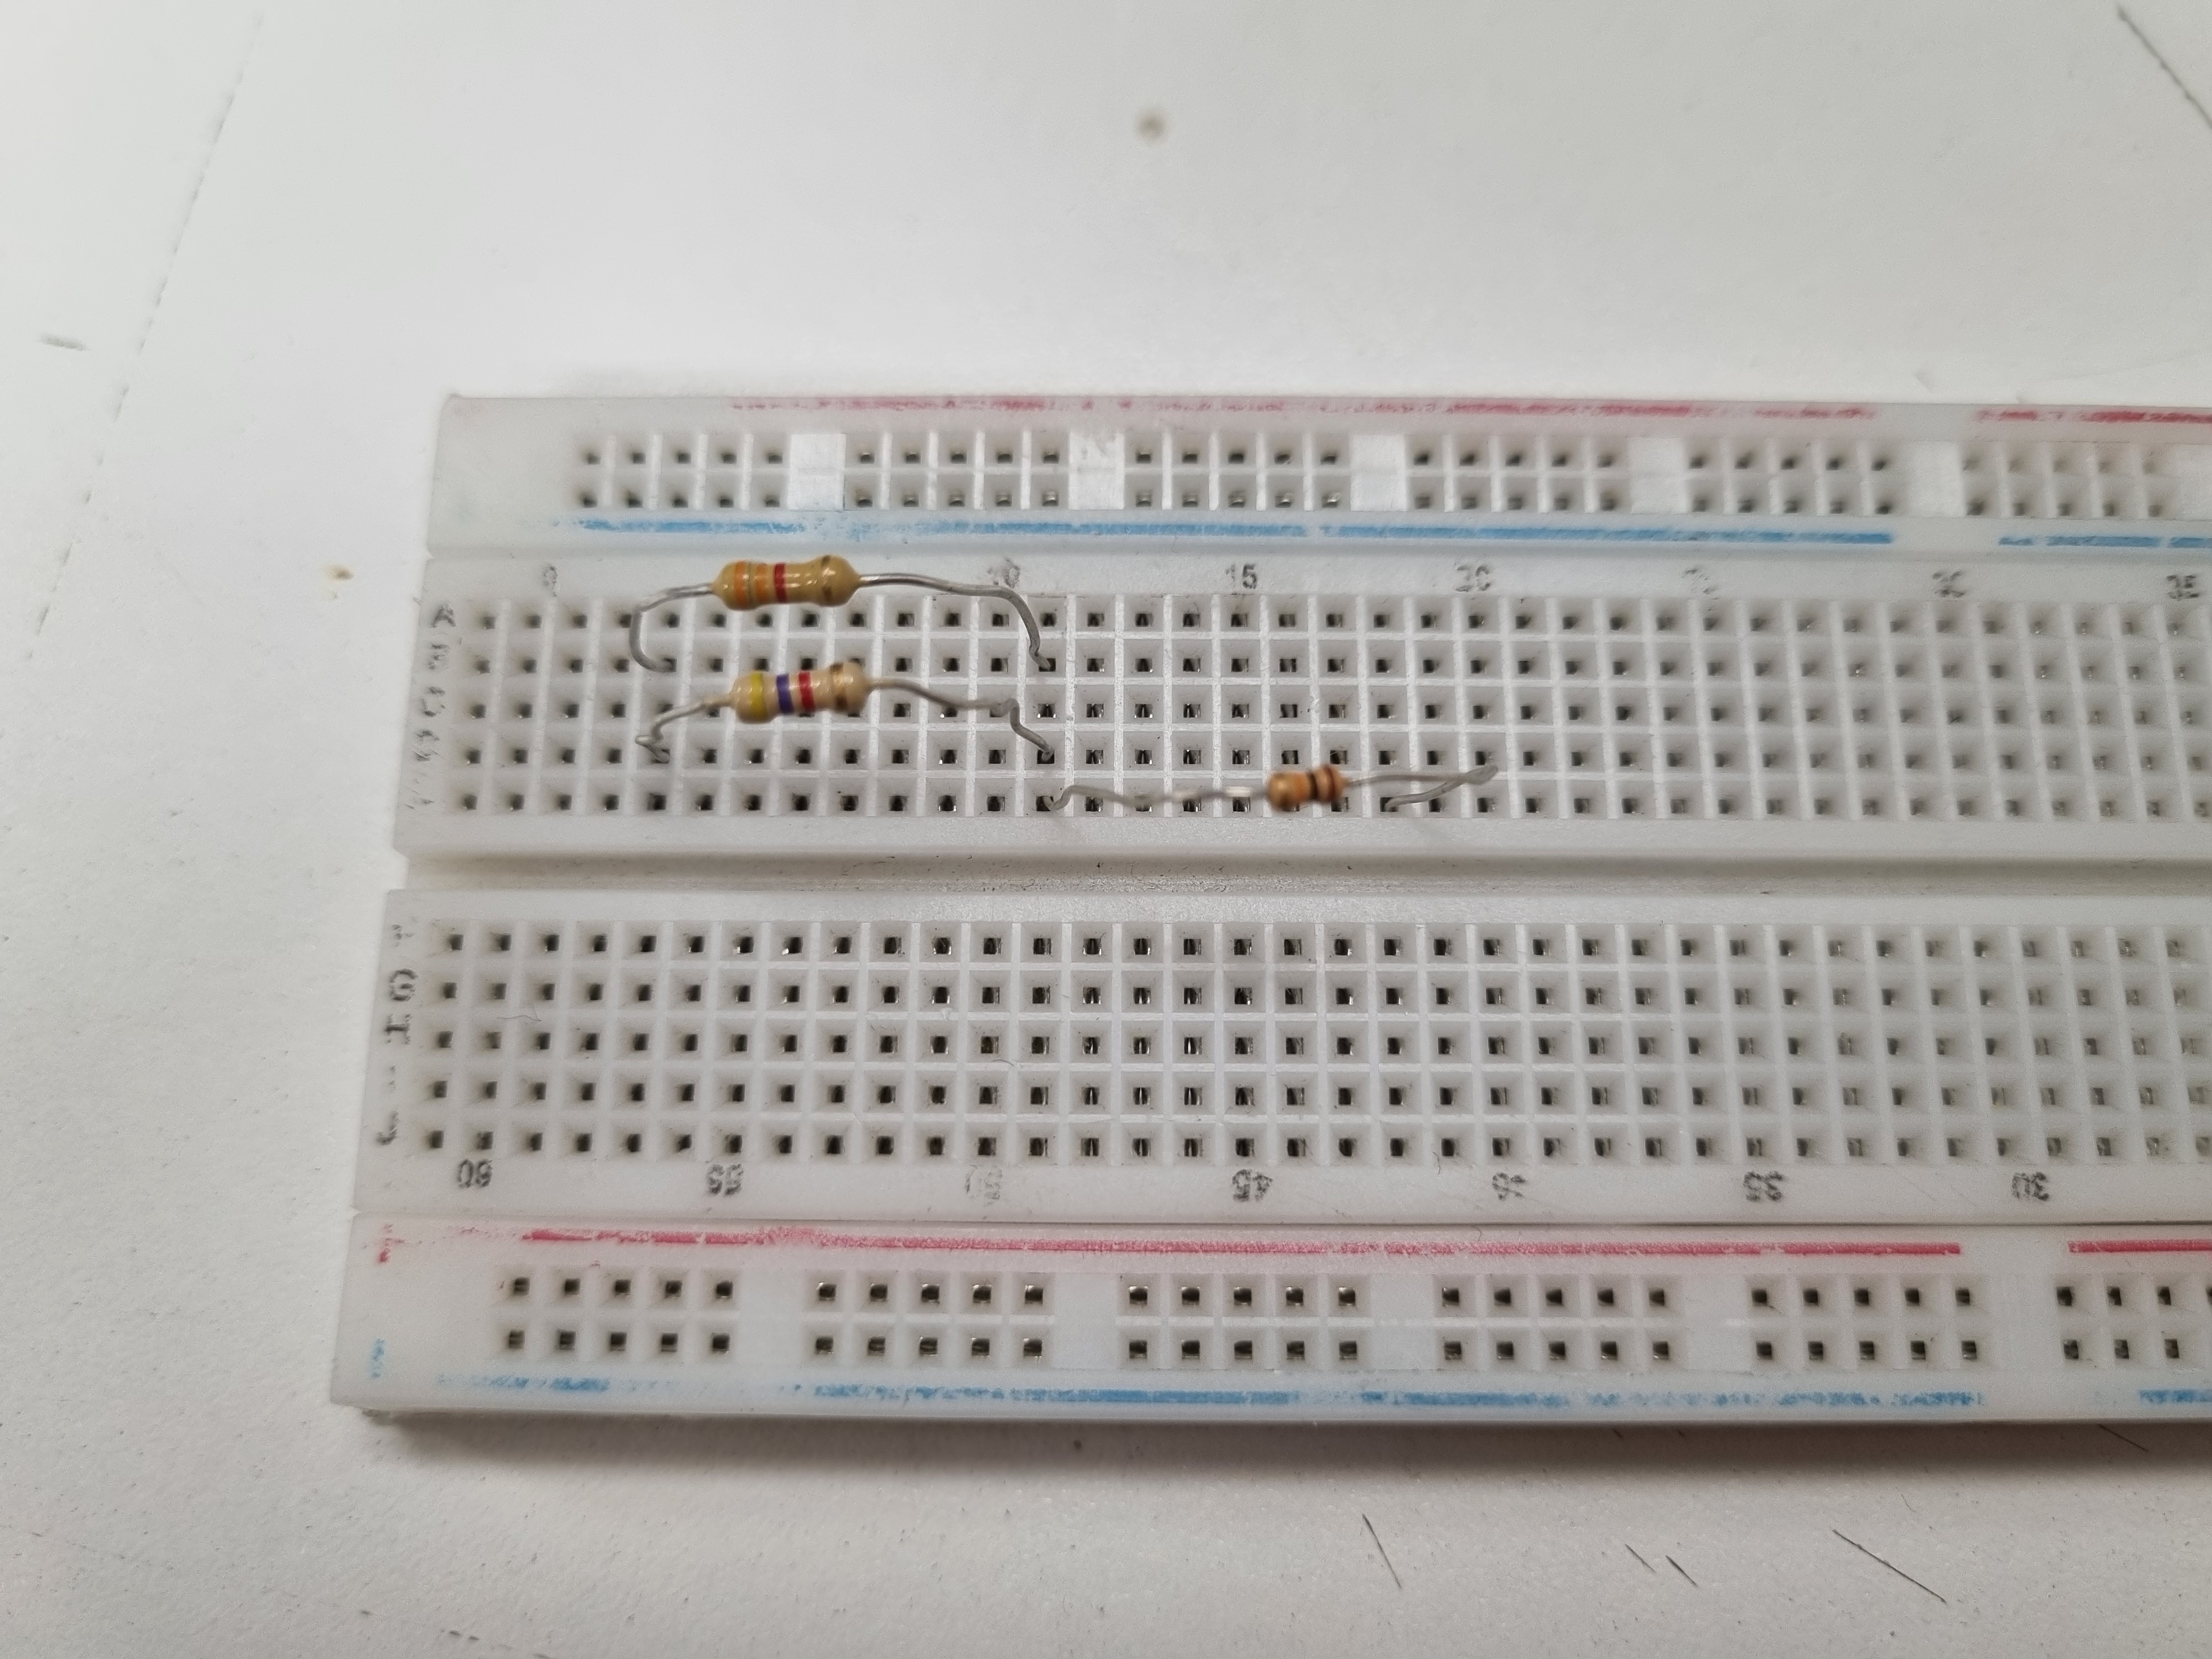
\includegraphics[width=\linewidth]{imagenes/proto.jpg}
        \caption*{Circuito armado en protoboard}
    \end{minipage}
\end{figure}

\paragraph{Mediciones de Tensión}
\paragraph{}

\begin{figure}[H]
    \centering
    \begin{minipage}{0.40\textwidth}
        \centering
        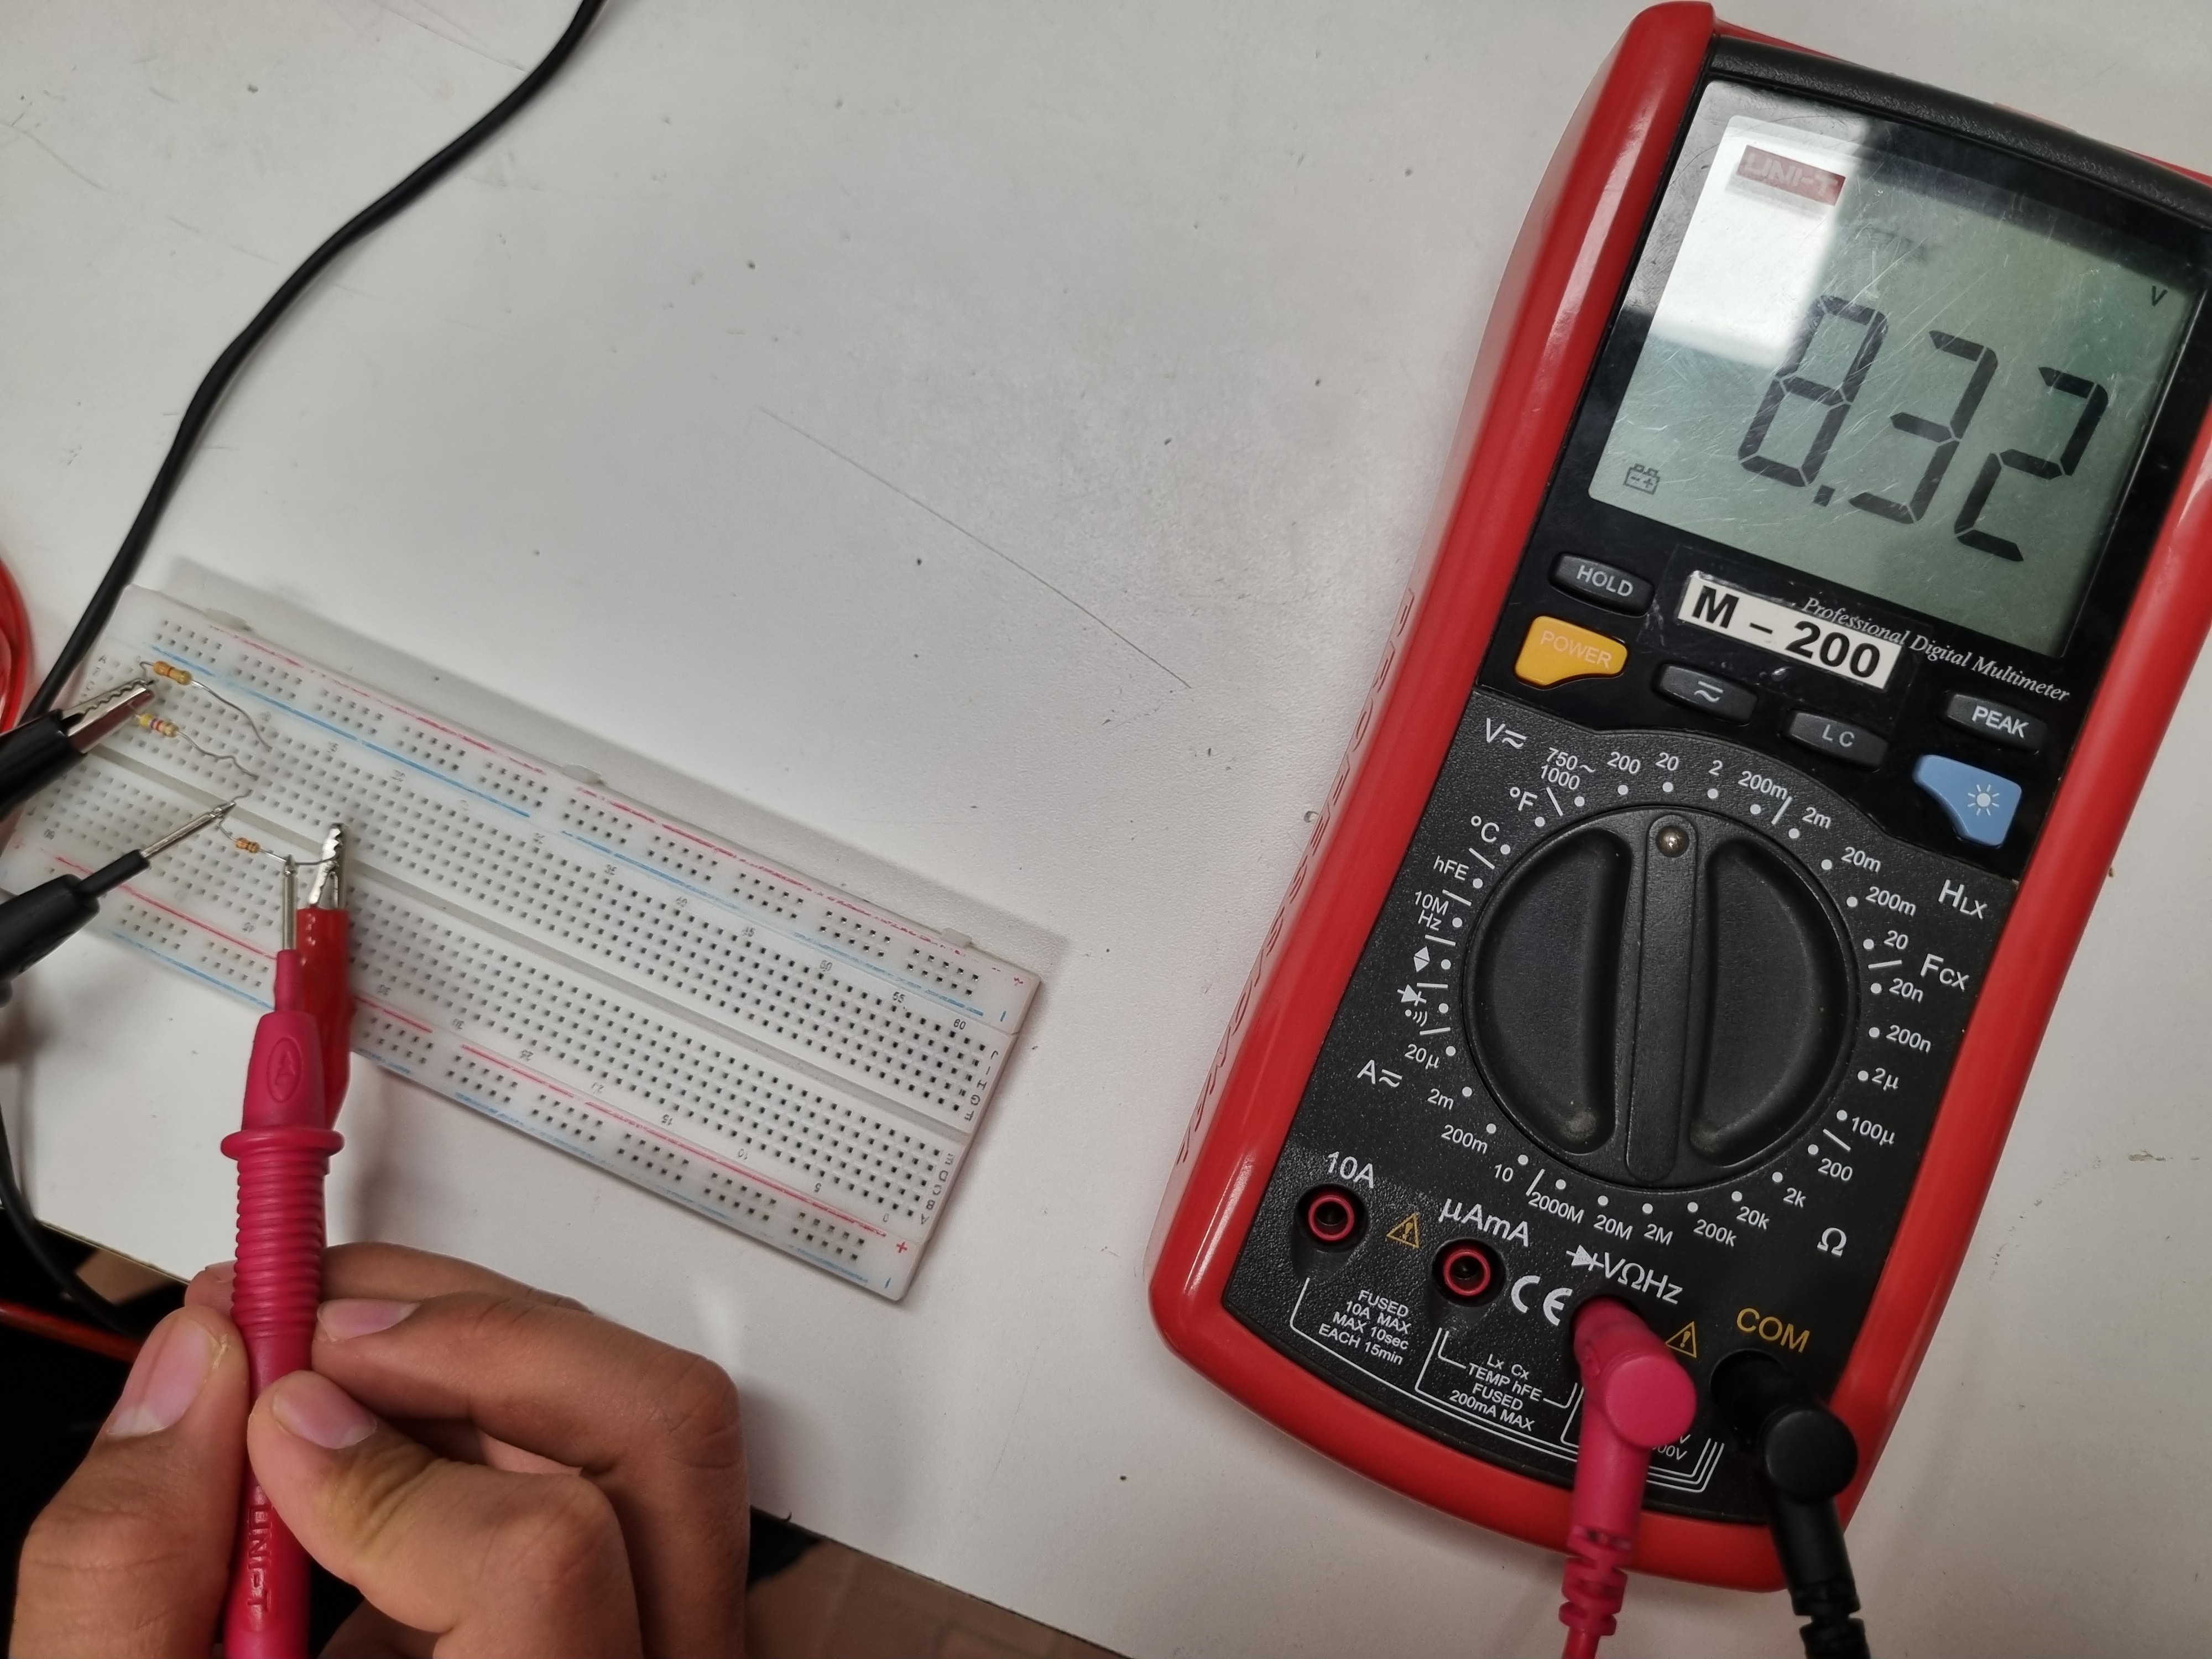
\includegraphics[width=\linewidth]{imagenes/tensioni1.jpg}
        \caption*{Tensión por $R_1$}
    \end{minipage}
    \hfill
    \begin{minipage}{0.40\textwidth}
        \centering
        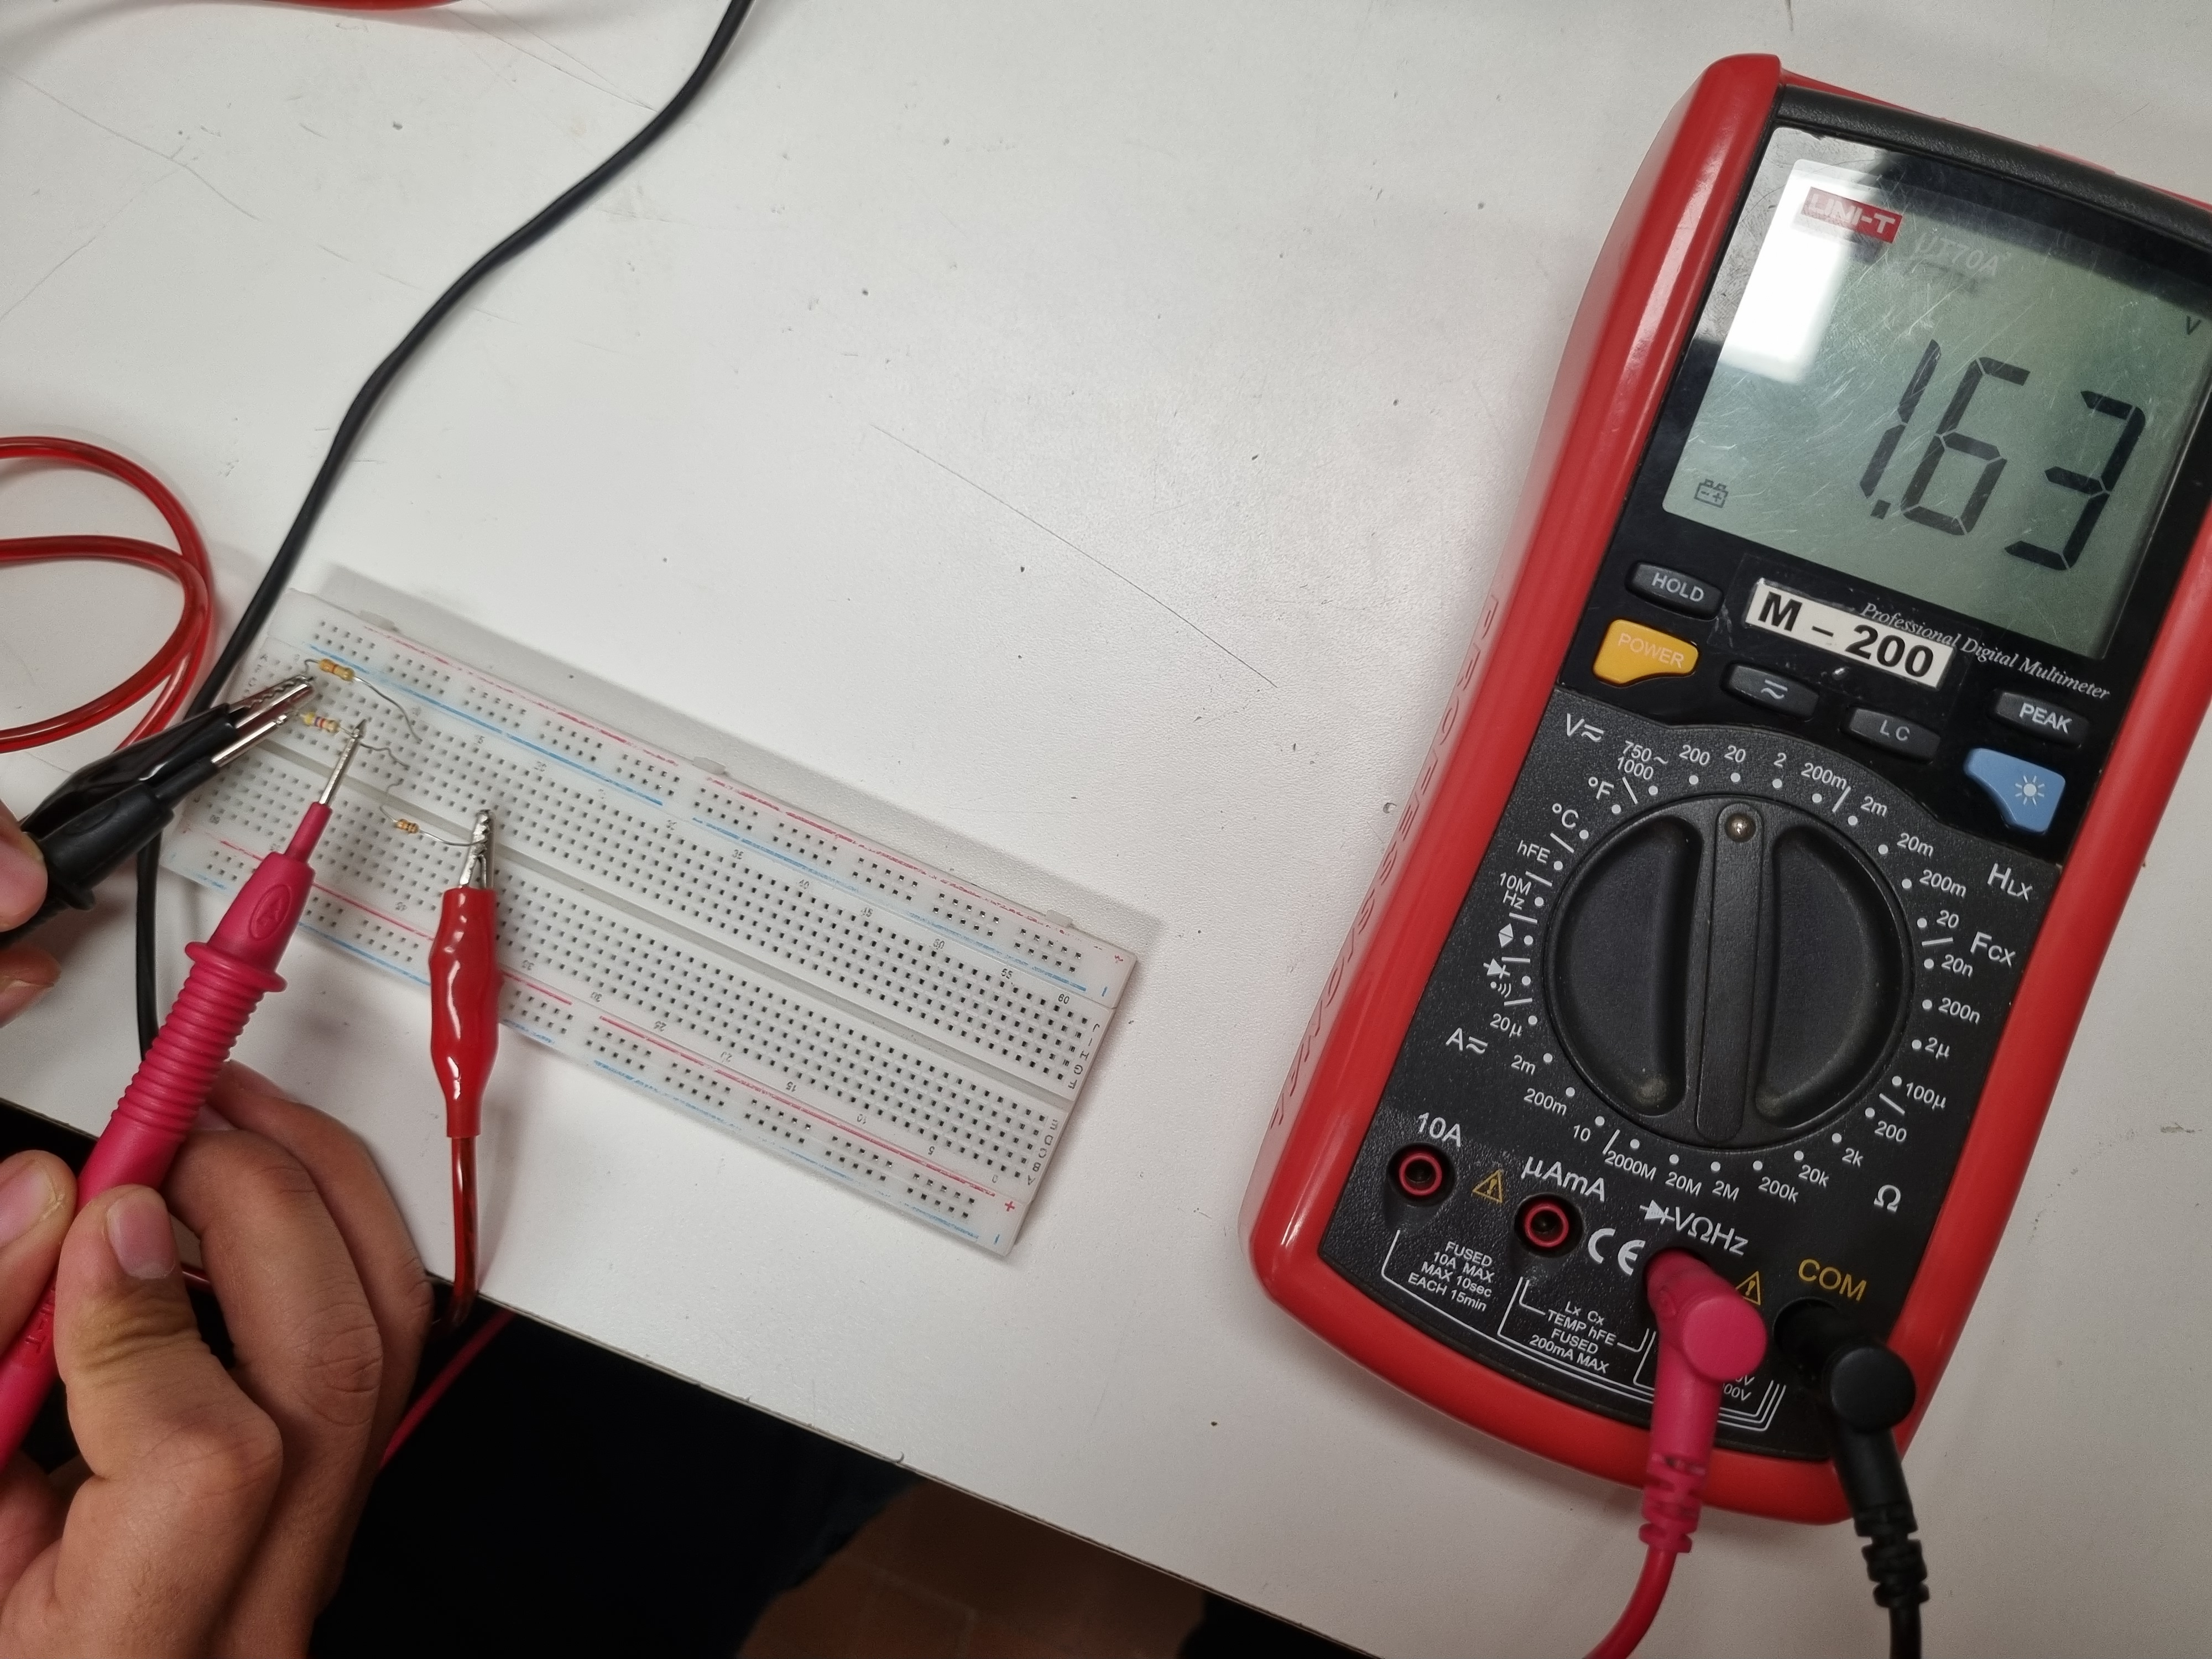
\includegraphics[width=\linewidth]{imagenes/tensioni2.jpg}
        \caption*{Tensión por $R_2$}
    \end{minipage}
\end{figure}

Como se menciono anteriormente al estar en paralelo la tensión por R3 será igual que por R2.

\vspace{9cm}

\paragraph{Mediciones de Corriente}
\paragraph{}

\begin{figure}[H]
    \centering
    \begin{minipage}{0.40\textwidth}
        \centering
        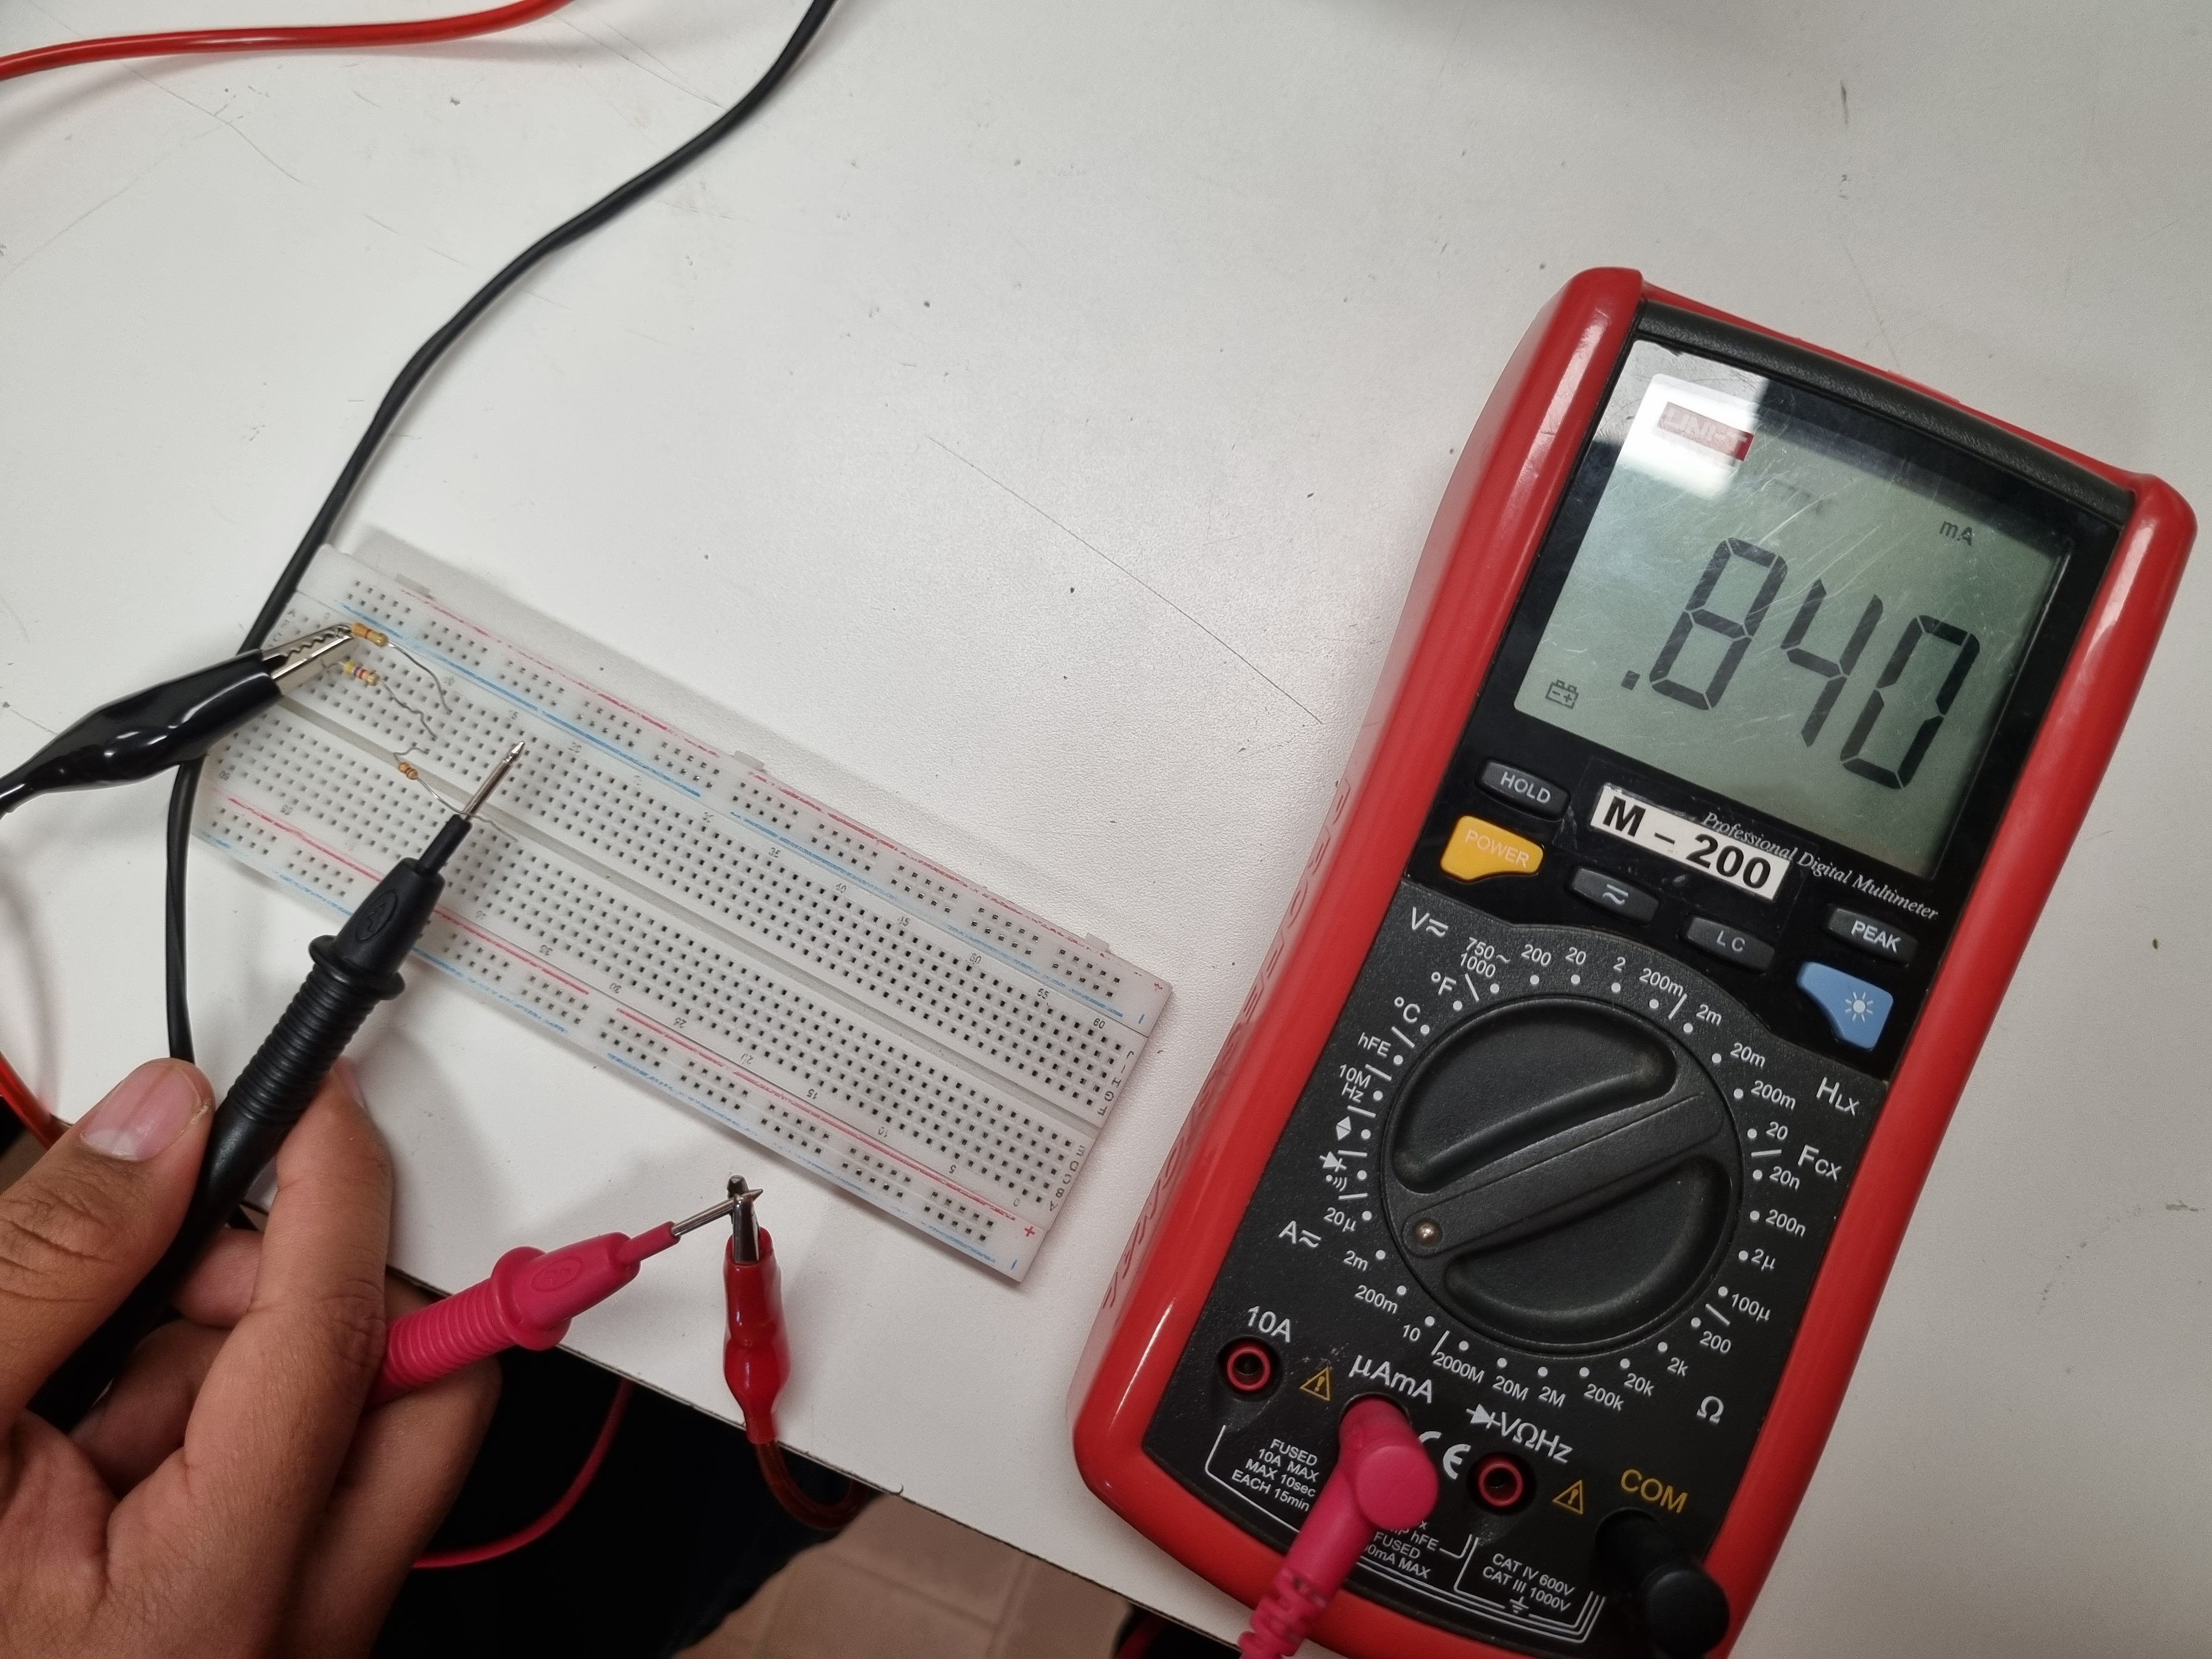
\includegraphics[width=\linewidth]{imagenes/corrientei1.jpg}
        \caption*{Corriente $R_1$}
    \end{minipage}
    \hfill
    \begin{minipage}{0.40\textwidth}
        \centering
        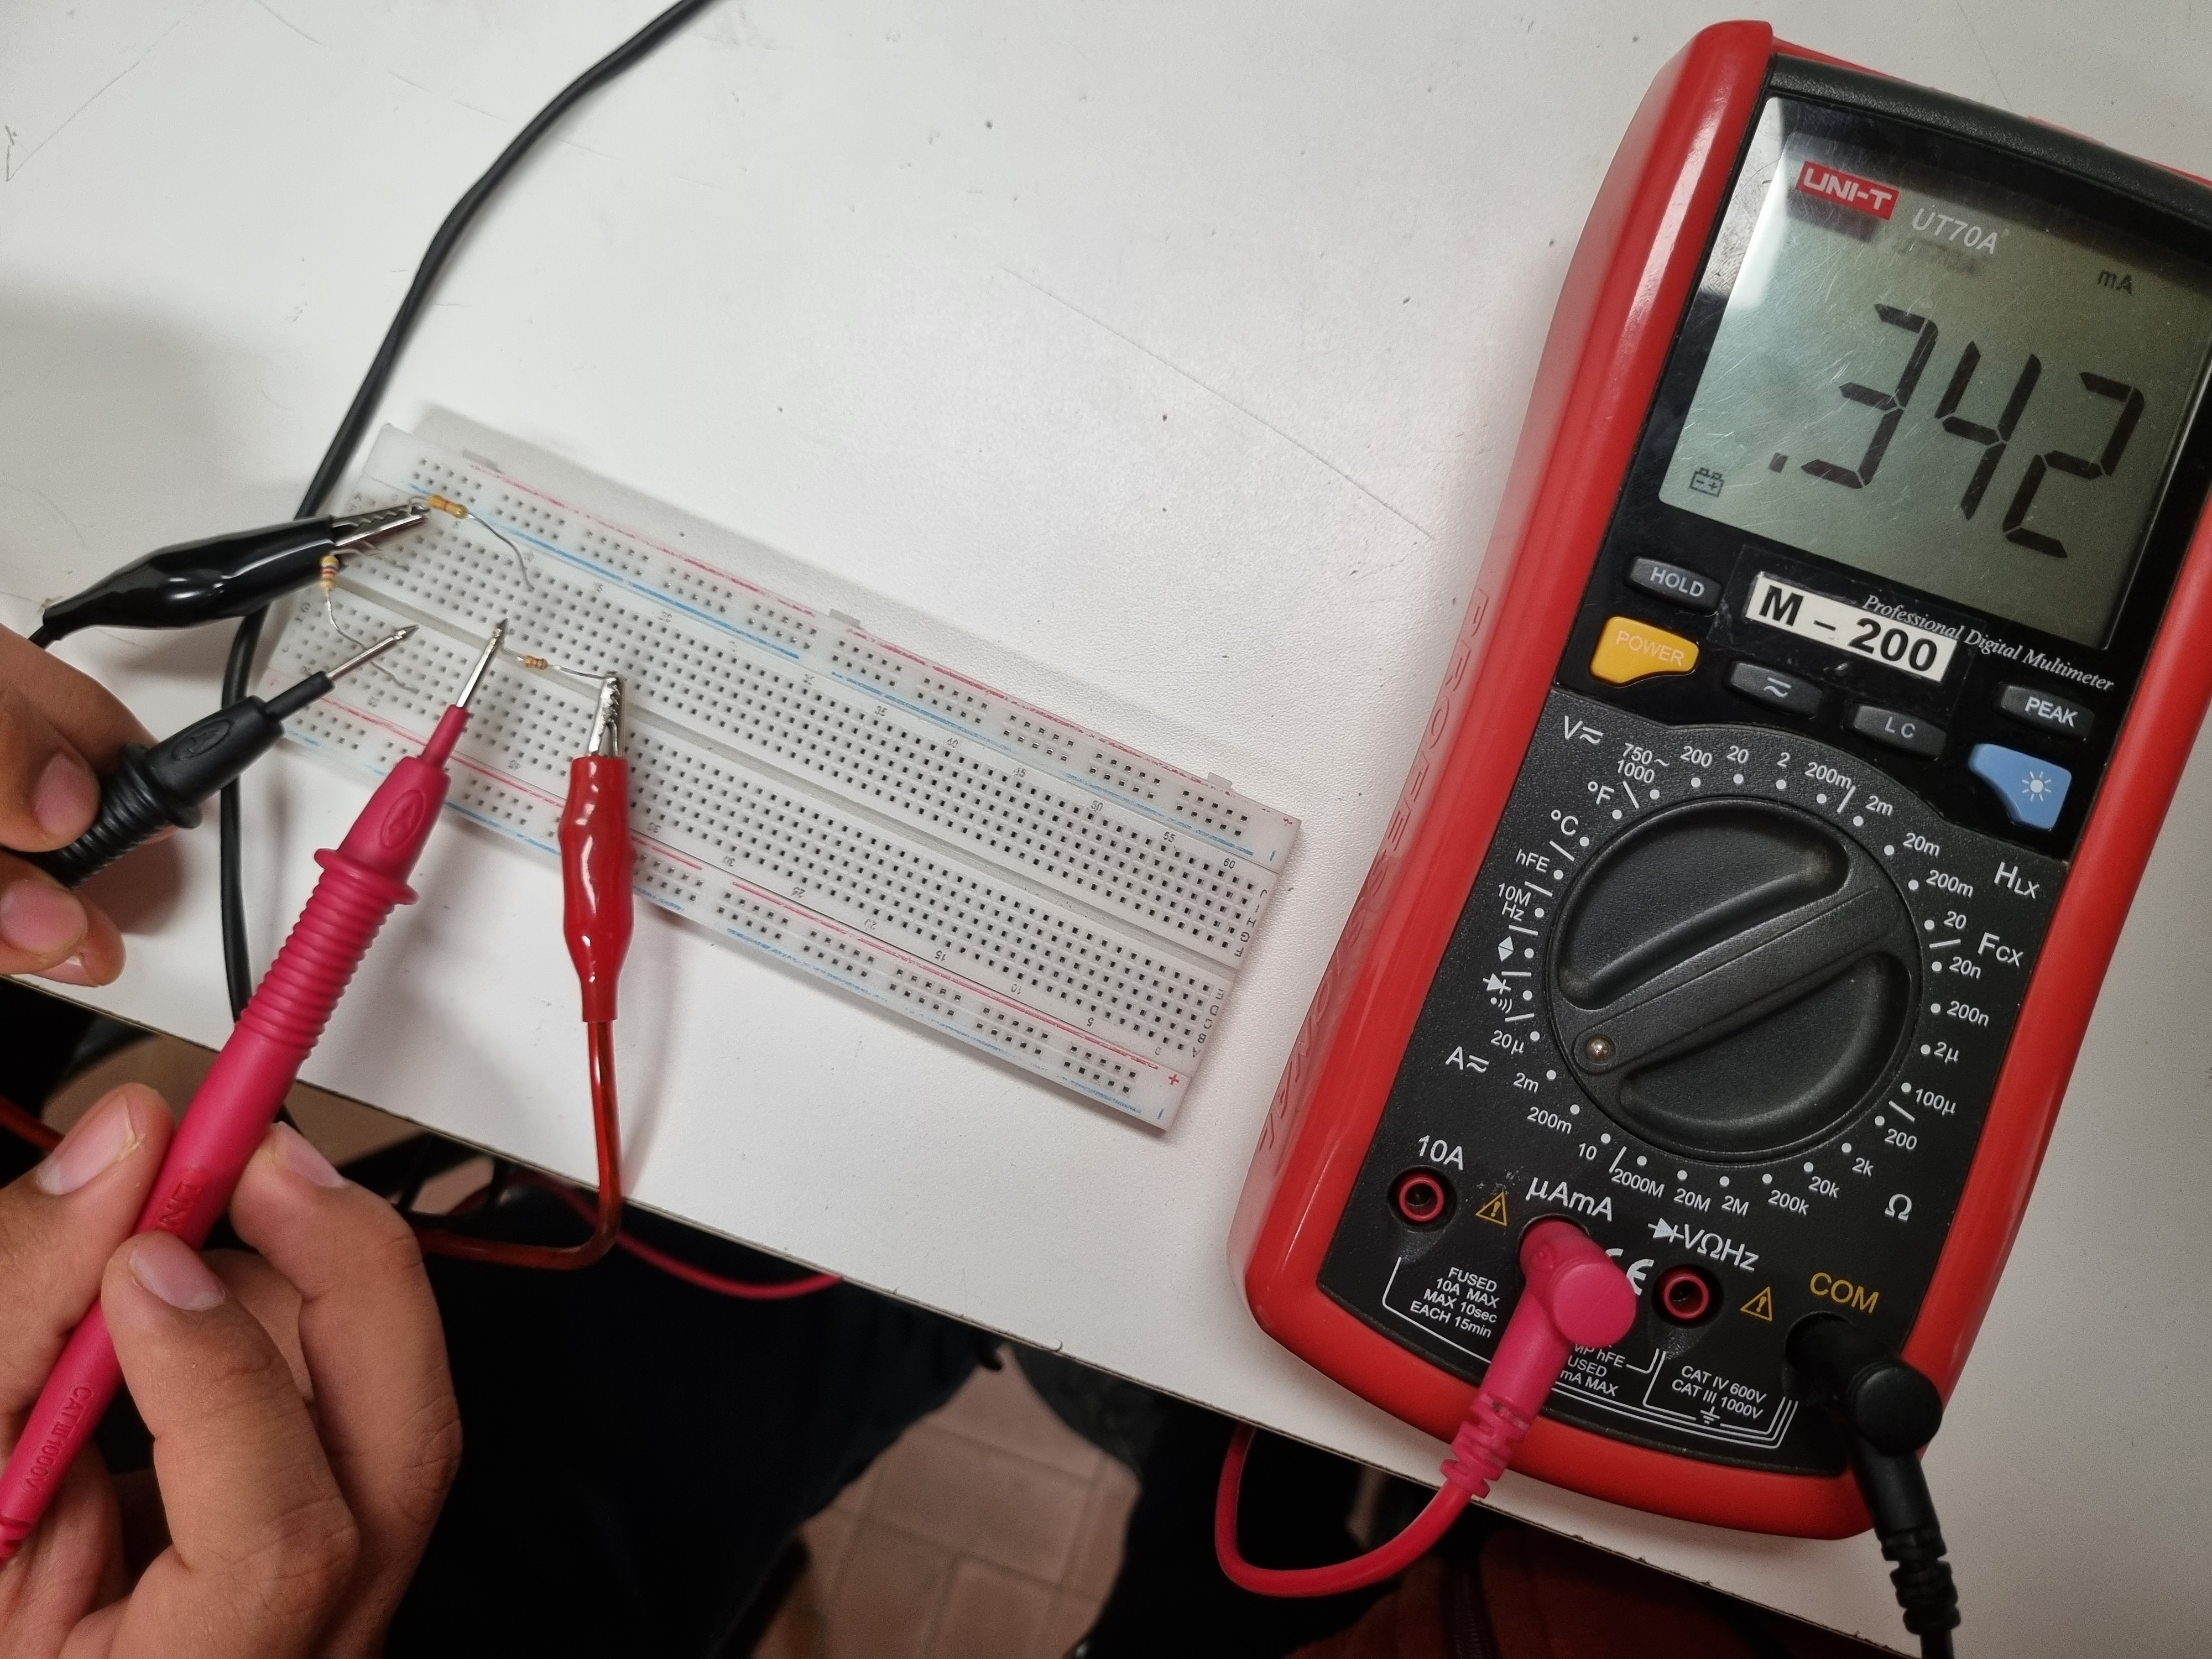
\includegraphics[width=\linewidth]{imagenes/corrientei2.jpg}
        \caption*{Corriente $R_2$}
    \end{minipage}
    \hfill
    \begin{minipage}{0.40\textwidth}
        \centering
        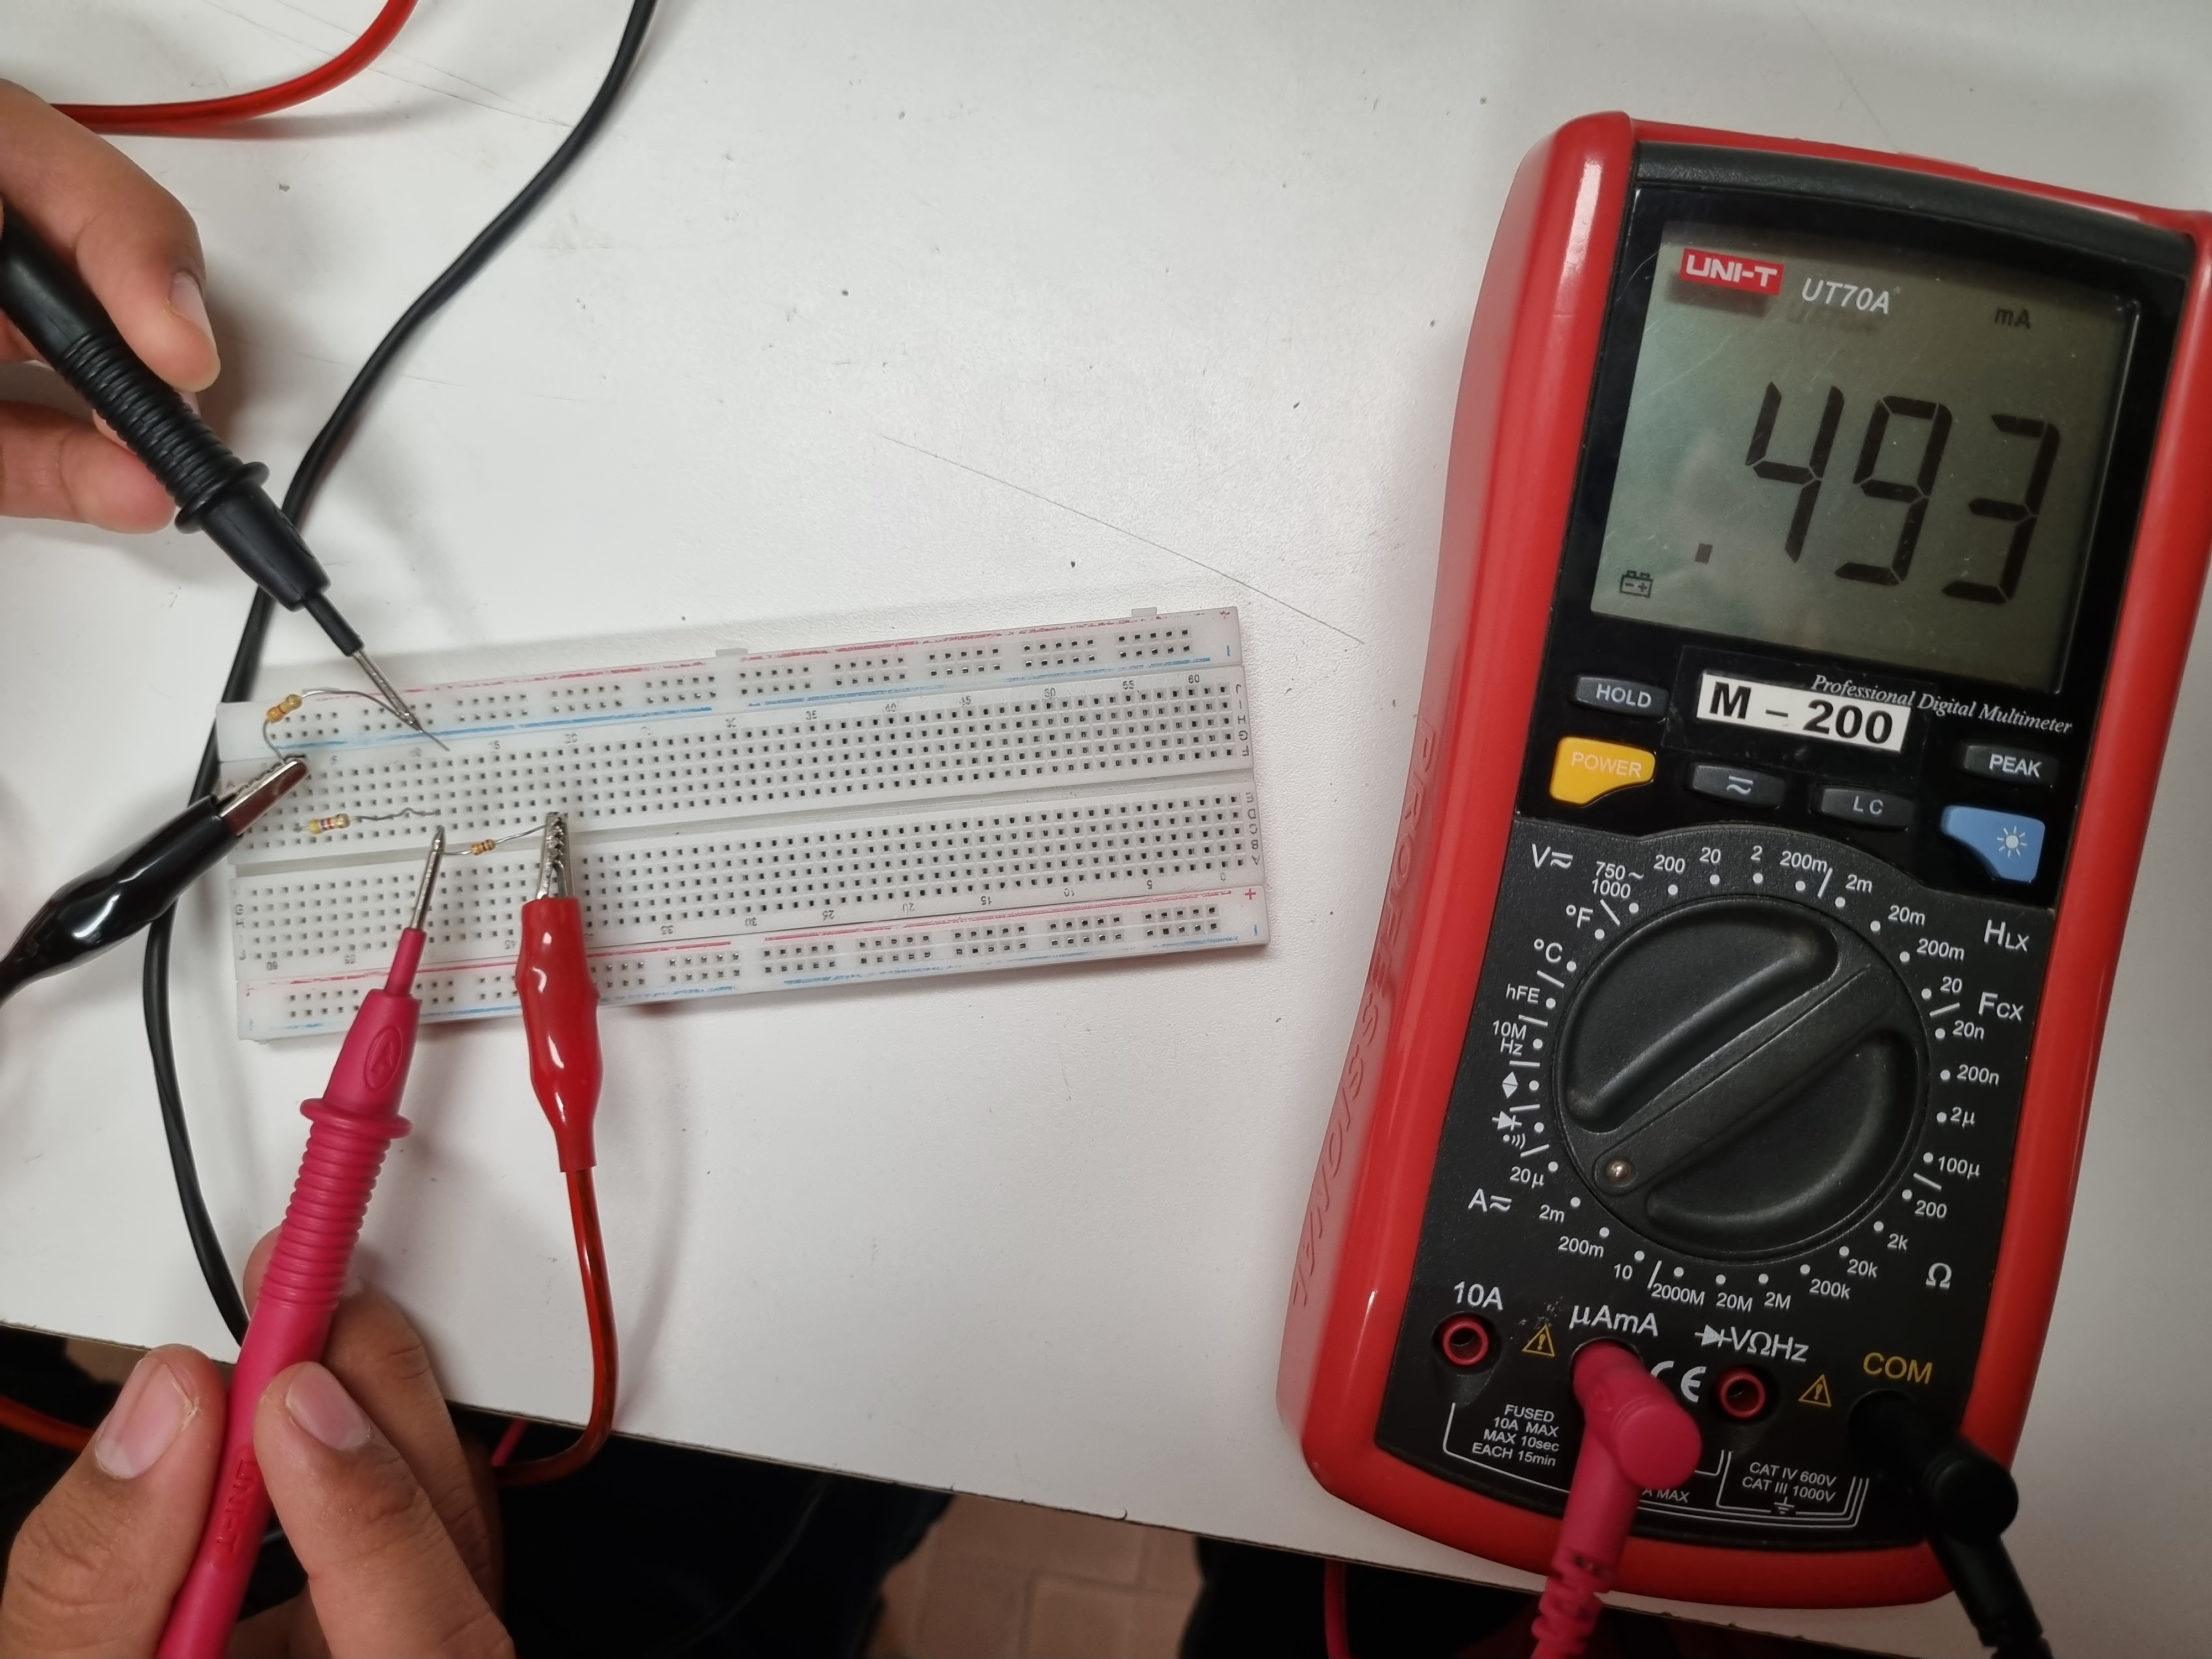
\includegraphics[width=\linewidth]{imagenes/corrientei3.jpg}
        \caption*{Corriente $R_3$}
    \end{minipage}
\end{figure}

\paragraph{Comparación de resultados:}
\paragraph{}

\begin{table}[H]
    \centering
    \begin{tabular}{|c|c|>{\centering\arraybackslash}p{0.1\linewidth}|>{\centering\arraybackslash}p{0.1\linewidth}|>{\centering\arraybackslash}p{0.1\linewidth}|>{\centering\arraybackslash}p{0.1\linewidth}|} \hline 
         &&  $V_s$&  $R_1$&  $R_2$& $R_3$\\ \hline 
         \multirow{3}{*}{Tensión} &  Análisis&  10 V&  8,37V&  1,63V& 1,63V\\ \cline{2-6}
         &  Simulación&  10 V&  8.37 V&   1.62 V& 1.62 V\\ \cline{2-6}
         &  Medición&  9.96 V&  8.32 V&  1.63 V& 1.63 V\\ \hline 
         \multirow{3}{*}{Corriente} &  Análisis&  $837,6 \mu A$&  $837,6 \mu A$&  $345.5 \mu A$& $492.1 \mu A$\\ \cline{2-6}
         &  Simulación&  $837.6 \mu A$&  $837.6 \mu A$&  $345.5 \mu A$& $492.1 \mu A$\\ \cline{2-6}
         &  Medición&  $840 \mu A$&  $840 \mu A$&  $342 \mu A$& $493 \mu A$\\ \hline
    \end{tabular}
\end{table}

\vspace{4cm}

\section{Conclusión}

\subsection{Conclusión A:}

Realizando los calculos respectivos de potencia, la cual es $P = I^2 \cdot R$, obtenemos como resultado para $R_1$ es $7mW$, para saber si fueron seleccionadas correctamente las potencias de los resistores utilizados, debemos considerar que el valor de la potencia sea menor a $\frac{1}{4}W$, la cual es la potencia de dichas resistencias. Podemos observar a simple vista que $7mW < 250mW$, por lo que si estan correctamente seleccionadas.

\subsection{Conclusión B:}

En el cuadro de comparación se observa una leve diferencia en la sección de medicion con respecto a la de análisis y la de simulación, esto esta bien y se debe a que en la medicion tenemos otros factores afectando que en el análisis y en la simulación no, tales como las tolerancias de los dispositivos, la precisión del multimetro que no es perfecta o que la fuente no es una fuente ideal, como en el analisis y simulaión.

\end{document}
